\documentclass[conference]{IEEEtran}

% The preceding line is only needed to identify funding in the first footnote. If that is unneeded, please comment it out.
\renewcommand\IEEEkeywordsname{Keywords}

\usepackage{caption}
\usepackage{url}
\usepackage{titletoc}
\usepackage{graphicx}
\usepackage[utf8]{inputenc}
\usepackage[T1]{fontenc}
\usepackage[table]{xcolor}
\usepackage{tabulary}

\usepackage{titlesec}
\def\thesubsubsectiondis{\unskip\arabic{subsubsection})}
\titlespacing*{\subsubsection}{0pt}{10pt plus 4pt minus 2pt}{4pt plus 2pt minus 2pt}

\usepackage{hyperref}
\hypersetup{
    colorlinks=true,
    linkcolor=blue,
    urlcolor=brown,
    }

% import math notations
\newcommand{\epoch}{\ensuremath{\epsilon}}

\newcommand{\work}{\ensuremath{W}}
\newcommand{\fee}{\ensuremath{F}}
\newcommand{\deposit}{\ensuremath{D}}

\newcommand{\node}{\ensuremath{N}}
\newcommand{\publicGoodNode}{\ensuremath{\node_p}}
\newcommand{\staking}{\ensuremath{s}}
\newcommand{\chip}{\ensuremath{C}}
\newcommand{\trust}{\ensuremath{t}}
\newcommand{\operation}{\ensuremath{o}}

\newcommand{\nodeAtEpoch}{\ensuremath{{\node,\epoch}}}


\newcommand{\pool}{\ensuremath{P}}

\newcommand{\stakingPool}{\ensuremath{\pool_\staking}}

\newcommand{\operationPool}{\ensuremath{\pool_\operation}}

\newcommand{\publicGood}{\ensuremath{p}}
\newcommand{\publicGoodPool}{\ensuremath{\pool_\publicGood}}

\newcommand{\networkReward}{\ensuremath{R}}

\newcommand{\stakingReward}{\ensuremath{\networkReward_\staking}}
\newcommand{\operationReward}{\ensuremath{\networkReward_\operation}}
\newcommand{\trustReward}{\ensuremath{\networkReward_\trust}}

\newcommand{\tax}{\ensuremath{T}}
\newcommand{\taxCap}{\ensuremath{c}}
\newcommand{\taxRate}{\ensuremath{\tau}}

\newcommand{\reliabilityScore}{\ensuremath{\sigma}}


\usepackage[nopostdot,automake]{glossaries-extra}

\usepackage{ifthen}

\setabbreviationstyle{long-short}
\setglossarystyle{altlist}

\makeglossaries
% only show link on first use
\GlsXtrEnableEntryUnitCounting{general}{0}{chapter}
\renewcommand*{\glslinkcheckfirsthyperhook}{%
    \ifnum\glsentrycurrcount\glslabel>0
        \setkeys{glslink}{hyper=false}%
    \fi
}

% #1 - short name: OIL
% #2 - math symbol
% #3 - full name: Open Information Layer
% #4 - description

\newcommand{\newdualentry}[4]{%
    \ifthenelse{\equal{#2}{}}%
    {
        % If #2 (the math symbol) is empty
        \newglossaryentry{#1}{%
            name={#3 - #1},
            text={#1},
            short={#1},
            long={#3},
            first={#3 (#1)},
            firstplural={#3s (#1s)},
            description={#4},
            sort={#1}
        }
    }{
        % If #2 is provided
        \newglossaryentry{#1}{%
            name={#3 - \ensuremath{#2}},
            text={#1},
            short={\ensuremath{#2}},
            long={#3},
            first={#3 (\ensuremath{#2})},
            firstplural={#3s (#1s)},
            description={#4},
            symbol={\ensuremath{#2}},
            sort={#1}
        }
    }
}

\newdualentry{OW}{}{Open Web}{The next-generation Internet where information flows openly without any restrictions, as it is supposed to be.}

\newdualentry{OI}{}{Open Information}{Information that is typically found across various types of networks, including decentralized, federated, and centralized networks that allow permissionless access.}

\newdualentry{OIL}{}{Open Information Layer}{A decentralized and permissionless information layer where information flows openly without any restrictions.}

\newdualentry{DSL}{}{Data Sublayer}{A decentralized network where the Open Information flows from its source to its destination.}

\newdualentry{Protocol}{}{RSS3 Protocol}{A unified set of data structures for interoperability.}

\newdualentry{Node}{\node}{Node}{A Data Sublayer component that indexes, cleans, stores, and ultimately serves the Open Information to the end users. Denoted as \node\ when it is in Normal mode, and \publicGoodNode\ when it is in Public Good mode.}

\newdualentry{SNP}{\publicGoodNode}{Node (Public Good Mode)}{A \gls{Node} that operates for the purpose of supporting Public Goods and strenthening the Network, it does not receive any \glsfmtlong{Fee} or \glsfmtlong{NR}.}

\newdualentry{RS}{\reliabilityScore}{Reliability Score}{A score used to determine the allocation of requests to \glsfmtlong{Node}s.}

\newdualentry{GI}{}{Global Indexer}{A \glsfmtlong{DSL} component that facilitates coordination among \glsfmtlong{Node}s and engages with the \glsfmtlong{VSL}.}

\newdualentry{VSL}{}{Value Sublayer}{A blockchain where the value created by Open Information activities is recorded and distributed.}

\newdualentry{PDS}{}{Permissionless Data Source}{A repository of data that can be accessed without the need for authorization or authentication.}

\newdualentry{NR}{\networkReward}{Network Rewards}{Tokens allocated by the RSS3 Network to incentivize network participants.}

\newdualentry{OR}{\operationReward}{Operation Rewards}{Tokens allocated to \glsfmtlong{OP} by the RSS3 Network to incentivize Node operation.}

\newdualentry{SR}{\stakingReward}{Staking Rewards}{Tokens allocated to \glsfmtlong{SP} by the RSS3 Network to incentivize network participation.}

\newdualentry{TR}{\trustReward}{Trust Rewards}{Tokens allocated to \glsfmtlong{PGP} by the RSS3 Network to incentivize network participation and support Nodes for Public Goods provision.}

\newdualentry{NO}{}{Node Operator}{An individual or organization that operates a Node.}

\newdualentry{PGP}{\publicGoodPool}{Public Good Pool}{A collective pool of staked \$RSS3 that is used to improve the RSS3 Network by assigning trust to Public Good Nodes.}

\newdualentry{OP}{\operationPool}{Operation Pool}{A pool of \$RSS3 that consists of 1) Fees collected from serving Data Sublayer requests; 2) \glsfmtlong{NR} allocated based on the Node's work; 3) Tax collected from its Staking Pool.}

\newdualentry{SP}{\stakingPool}{Staking Pool}{A pool of staked \$RSS3 that is used to improve the RSS3 Network by assigning trust to Normal Nodes.}

\newdualentry{R3N}{}{RSS3 Network}{A decentralized network that is formed by a DSL and a VSL.}

\newdualentry{Epoch}{\epoch}{Epoch}{A period of time used as a reference to measure the \glsfmtlong{R3N}'s operation.}

\newdualentry{N}{\work}{number of requests served on the \glsfmtlong{DSL}}{The metric that reflects the Node's service and is used to determine the allocation of \glsfmtlong{NR} into a Node's \glsfmtlong{OP}.}

\newdualentry{Tax}{\tax}{Operation Tax}{A tax collected from the \glsfmtlong{NR} that are allocated to a Node's \glsfmtlong{SP}, by its \glsfmtlong{OP}.}

\newdualentry{Deposit}{\deposit}{Deposit}{Tokens required to operate a \glsfmtlong{Node}.}

\newdualentry{Fee}{\fee}{Request Fees}{Fees paid to \glspl{Node} for delivering \glsfmtlong{OI} from its \glsfmtlong{PDS} to the requesters.}

\newdualentry{Chip}{\chip}{Chip}{An ERC-721 Non-Fungible Tokens (NFTs) representing a network participant's stake in a particular Node.}

\newdualentry{Slashing}{}{Slashing}{A penalty imposed on a Node for misconduct.}

\newdualentry{REP}{}{RSS3 Evolution Proposal}{The proposal to change the RSS3 Network's parameters, processes and rules.}


\usepackage[nameinlink]{cleveref}

\begin{document}

\title{RSS3: The Open Information Layer}

\author{Natural Selection Labs}
\maketitle

\thispagestyle{plain}
\pagestyle{plain}
\pagenumbering{arabic}

\begin{abstract}

    Inspired by the original RSS Standard, this paper presents RSS3, the \glsfmtlong{OIL} for the \glsfmtlong{OW}. The paper serves as an enhanced version of our initial whitepaper titled ``RSS3: A Next-Generation Feed Standard.'' Following the release of our initial whitepaper, we have adhered to its proposed architecture to conduct experiments and advance the development of the RSS3 Network. The Network has transformed into what is now known as the \glsfmtlong{OIL}, reflecting the evolving dynamics of the \glsfmtlong{OW}. This paper summarizes our research and development output since then, providing insights into RSS3's vision and its decentralization architecture. Finally, we present the Network's tokenomics and governance model, and discuss the future of RSS3.

\end{abstract}

\section{Introduction}

RSS3 is the \glsfmtlong{OIL}, structuring \glsfmtlong{OI} for social, search, and AI.
The \gls{OIL} is a decentralized and permissionless layer where information flows openly without any restrictions, as it is supposed to be.

It is RSS3's mission to construct the \glsfmtlong{OW} by enhancing the free flow of \glsfmtlong{OI}.



\section{\glsfmtlong{R3N}}

The \glsfmtlong{R3N} is a decentralized network that is formed by two Sublayers: the \glsfirst{DSL} and the \glsfirst{VSL}.
This novel network structure is the product of a series of research and development experiments, that were conducted to address the challenges faced by the Open Web.

\gls{OI} is typically found across various types of networks, including decentralized, federated, and centralized networks that allow permissionless access.
The \gls{DSL} is responsible for indexing and structuring \gls{OI} for interoperability.
This is achieved by introducing a crucial standard, known as the \gls{UMS}, see \Cref{subsec:UMS}, enabling network-agnostic applications to be built on top of the \gls{DSL}.
The \gls{DSL} then leverages the \gls{VSL}, see \Cref{sec:VSL}, to build an ownership economy for the \gls{OW}.

\subsection{\$RSS3}
\$RSS3 is the Network's native utility token. It is used to cover gas, pay request fees, operate nodes, participate in staking and trust, distribute incentives, and engage in various network activities. See \Cref{sec:tokenomics} for more details.

\subsection{\Glsfmtfull{Epoch}}

An \glsfirst{Epoch} is a period of time used as a reference to measure the RSS3 Network’s operation, during which the Network's parameters are fixed.
The duration of an epoch is determined by the Network, and is subject to potential future changes.

At the end of each \epoch, the Network will distribute the \gls{NR} to the \glsfmtlong{R3N}'s participants, and update the Network's parameters when necessary.

\section{\glsfmtlong{DSL}}
\label{sec:DSL}

The \glsfirst{DSL} is responsible for \glsfmtlong{OI} life cycle management, which includes indexing, transformation, storage, dissemination, and consumption \cite{nationalinstituteofstandardsandtechnology2016Information}.
In this section we introduce the \gls{DSL} and its fundamental components, see \Cref{fig:DSL}.

The \gls{DSL} is formed by two components (see \cref{subsec:SN} and \cref{subsec:GI}), and uses the \gls{UMS} (see \cref{subsec:UMS}) to structure the information for applications in social, search, AI and beyond.

    {
        \begin{figure}[tb!]
            \centering
            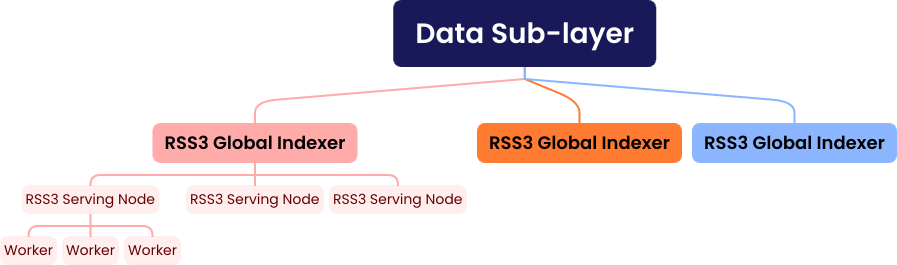
\includegraphics[width=\columnwidth]{figures/DSL.png}
            \caption{A topology of the \glsfmtlong{DSL}.}
            \label{fig:DSL}
        \end{figure}
    }


    {
        \begin{figure}[tb!]
            \centering
            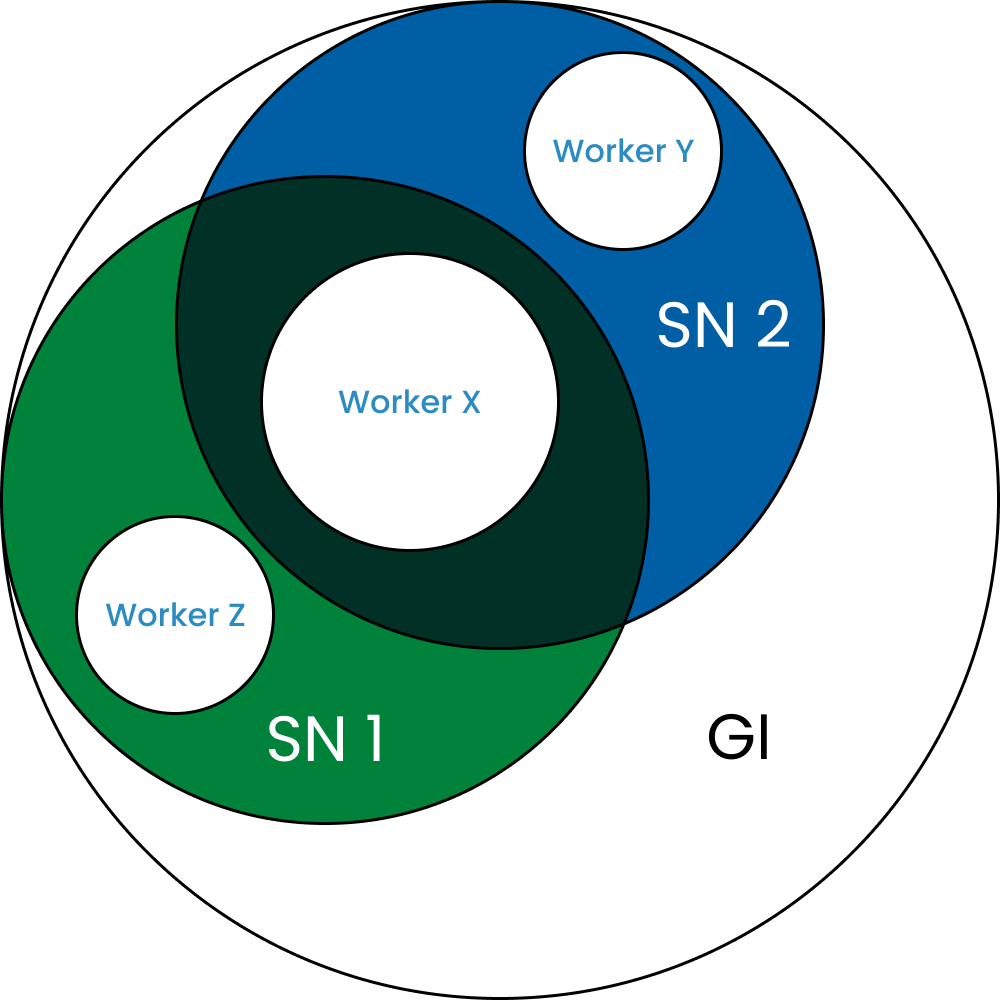
\includegraphics[width=0.7\columnwidth]{figures/GI.png}
            \caption{A venn diagram illustrating the relationship between the worker, the \glsfmtlong{SN} and the \glsfmtlong{GI}.}
            \label{fig:GI}
        \end{figure}
    }


\subsection{RSS3 \glsfmtfull{SN}}
\label{subsec:SN}

An \gls{SN}, also known as an RSS3 Node, is responsible for indexing, transforming, storing, and ultimately serving the \glsfmtlong{OI} to the end users.

The operation of an \gls{SN} is permissionless, and is subject to a set of requirements set by the Network.

\subsubsection{Indexing}
Each \gls{SN} operates a number of workers that index and structure \gls{OI} from \gls{PDS}.
Workers are community-maintained ``rules'' that define how \gls{OI} is indexed and transformed into the \gls{UMS} format.

Since each \gls{SN} is independent, it is possible for different \glspl{SN} to employ different combinations of workers to cover different \glspl{PDS}.
This design enables node operation to be flexible, accessible and affordable, in turn, offering a high degree of decentralization and robustness.

\subsubsection{Serving}
Each \gls{SN} operates a standard set of interfaces that serve structured \gls{OI} in \gls{UMS} to the end users via an \gls{GI}.

Each successful request served on the \gls{DSL} is recorded and the corresponding fees paid by the requesters are distributed to the \gls{SN}, see \Cref{subsubsec:operation_pool} for more details.

\subsection{RSS3 \glsfmtfull{GI}}
\label{subsec:GI}

A \gls{GI} is responsible for facilitating coordination among \glspl{SN} and engaging with the \gls{VSL}, and performs critical functions to ensure the \gls{DSL} is robust and reliable.

Given the importance of the \gls{GI} to the Network, its operation is not permissionless and is subject to a set of stringent requirements set by the Network.

\subsubsection{Performance Assurance} A GI acts as a load balancer and query router for end users to retrieve information from \glspl{SN}.
The unique architecture of the \gls{DSL} demands \glspl{GI} to be equipped with more computational capabilities, in order to work out the optimal route for end users to retrieve specific information from \gls{SN}, and frequently from a group of \glspl{SN} simultaneously.

\subsubsection{Quality Assurance} A GI acts as a supervisor for \glspl{SN} to ensure the quality of service.
With the \gls{DSL} being a permissionless sub-layer, the quality needs to be maintained strictly to ensure \glsfmtlong{R3N}'s robustness and reliability.
A \gls{GI} monitors the quality of \glspl{SN}, and slashes the \gls{SN} if it fails to meet the requirements.

\subsubsection{Proof-on-Chain} A GI keeps track of the work and slash records of \glspl{SN}, and submits them to the \gls{VSL} for settlement and reward allocation.

\subsection{Reliability Score} 

A \gls{GI} routes requests to \glspl{SN} based on their information coverage and a \gls{RS}.

\subsection{\glsfmtfull{UMS}}
\label{subsec:UMS}

Open Information, indexed from multiple \glspl{PDS}, is structured by \glspl{SN} into the \gls{UMS} format for interoperability.

\glspl{PDS} use different data structures, within a \gls{PDS}, there might be multiple products, services and protocols that leverage a different data structure to suit their needs.
This means limited interoperability, and developers need to look into each and every data structure, when it comes to building.
This lack of standardization means developers must investigate each unique structure individually when building applications, which is not scalable.

The \gls{UMS} addresses this issue by offering a unified set of data structures that serve as an abstraction.
This abstraction simplifies the integration process, making it more manageable and scalable for developers to work with data across various data sources.

For the complete set of the \gls{UMS}, refer to \url{https://docs.rss3.io/docs/unified-metadata-schemas}.



\section{\glsfmtlong{VSL}}
\label{sec:VSL}



The \glsfirst{VSL}, commonly referred to as the RSS3 Chain, is an Ethereum Layer 2 blockchain built with OP Stack using Celestia as the data availability layer.
It is responsible for handling value derived from \glsfmtlong{OI} activities and applications, establishing a healthy ownership economy for the Network.

In this section, we focus on the intentions behind the \gls{VSL}'s incentive mechanism, which is designed to promote stable Node Operations to maintain the Network, and to encourage network participants to secure the Network via staking \$RSS3.
We introduce the detailed tokenomics separately in \Cref{sec:tokenomics}.

The \glsfmtlong{R3N} allocates a portion of \$RSS3's total supply to incentivize network participants, referred to as the \glsfirst{NR},
are allocated into reward pools: the \glsfirst{SP} for Normal Nodes, or the \glsfirst{PGP} for Public Good Nodes.
See \Cref{fig:network-rewards} for an illustration and \Cref{subsec:reward_pools} for details on Reward Pools.
The calculations of \glsfmtlong{NR} are described in \Cref{subsec:network_rewards}.

\subsection{Node Operation}
\Glsfmtlong{NO}s are incentivized to operate and maintain the Network by receiving \$RSS3 as rewards.
\begin{enumerate}
    \item Anyone can become a \glsfmtlong{NO} to launch an RSS3 Node and join the RSS3 Network without requiring prior permission.
    \item A \glsfmtlong{NO} has the ability to configure Node's coverage, which directly influences the Node's capability to respond to various types of requests. A broader coverage means more computational resources are required, and an increased likelihood of receiving requests.
    \item A Node can be operated in either a Normal mode as \node, or a Public Good mode as \publicGoodNode. A Normal Node is eligible for \glsfmtlong{NR}, but requires a deposit of \$RSS3 into its \operationPool. A Public Good Node is ineligible for \glsfmtlong{NR}, but requires no deposit.
    \item A Normal Node has a corresponding \operationPool\ and a \stakingPool. All Public Good Nodes collectively share a single \publicGoodPool.
\end{enumerate}

\subsection{Node Staking}
Network participants are incentivized to stake \$RSS3 to secure the Network by receiving \$RSS3 as rewards.
\begin{enumerate}
    \item A Normal Node accepts staking into its \stakingPool, the amount of staked \$RSS3 signifies its quality. Higher quality Nodes has an increased likelihood of receiving requests.
    \item A Public Good Node does not have Reward Pools and does not participate in any form of incentivization. Staking into a \glsfmtlong{PGP} is accepted, and the stakers can assign their trust to any Public Good Node. Higher trust Nodes has an increased likelihood of receiving requests.
\end{enumerate}

{
\renewcommand{\arraystretch}{1.5}
\begin{table*}[h]
    \resizebox{\textwidth}{!}{
        \begin{tabulary}{\textwidth}{|p{6cm}|p{5cm}|p{5cm}|}
            \hline
            & \textbf{Node in Normal Mode} & \textbf{Node in Public Good mode} \\ \hline

            Who can operate? &
            Anyone &
            Anyone \\ \hline

            Is a deposit required for operating a Node? &
            Yes &
            No \\ \hline

            Is the deposit considered as staking, making it eligible for rewards from its own \stakingPool? &
            No &
            N/A \\ \hline

            Will the Node be slashed? &
            Yes, its deposit and \stakingPool will be slashed. A Node may be demoted to receive fewer requests.
            & No, but a Node may be demoted to receive fewer requests. \\ \hline

            Does the Node accept staking? &
            Yes. The staked tokens go to the Node’s \stakingPool. RSS3-X (X being the Node’s name) Chips are issued to the stakers after staking. &
            No, as such a Node does not have a \stakingPool. Instead, stakers stake to the \publicGoodPool. RSS3-Public Good Chips are issued to the stakers after staking. \\ \hline

            Can the \glsfmtlong{NO} set a tax \taxRate? &
            Yes &
            No, a universal tax is determined by the Network. \\ \hline

            Does it have an \glsfmtlong{OP} \operationPool? &
            Yes &
            No, its \glsfmtlong{OR} go to [X] \\ \hline

            Does it have a \glsfmtlong{SP} \stakingPool? &
            Yes &
            No, but a \glsfmtlong{PGP} with a universal incentive rate. \\ \hline
        \end{tabulary}
    }
    \caption{Comparison of two Node Operation modes.}
    \label{table:node_modes}
\end{table*}
}


\section{Conclusion} 

\textbf{At the heart of Natural Selection Labs, we firmly believe in the freedom of information distribution: No organizations or authorities shall prohibit the free exercise of the right of people to create, store, and distribute their information.}


\printglossary[type=main,title=Glossary, toctitle=Glossary]



\bibliographystyle{plain}
\bibliography{references}

\end{document}

